

\section{Background}

%%%%%%%%%%%%%%%%%%%%%%%%%%%%%%%%%%%%%%%%%%%%%%%%%%%%%%%%%%%%%%%%%%%%%%%%%%%%%%%%
\subsection{Terminology and Conventions}

Let $n,n_1,n_2 \in \NN$ such that $n_1 < n_2$. We often denote by $[n]$ to the set $\{1,2,\dots, n\}$ and by $[n_1,n_2]$ to the set $\{n_1, n_1+1, \dots, n_2 - 1, n_2\}$.

We denote by $\FF$ to a finite field of prime order $p$ and by $\FF^*$ to its respective multiplicative group. We also write $\FF[X]$ for the ring of polynomials with coefficients over $\FF$ and write $\FF_{<d}[X]$ to denote the set of polynomials of degree lower than $d$. Given a positive integer $N$, we always assume the existence of a cyclic subgroup $G$ of $\FF^*$ and denote by $g \in \FF$ to its generator.

In PIL we treat polynomials and entire columns of execution traces indistinguishably for the following reason. Given a column $\att$ of length $N$, which can be viewed as the vector $(a_1,\dots,a_N)$ with $a_i \in \FF$ for $i \in [N]$, we define the polynomial $\att(X) \in \FF_{<N}[X]$ such that $\att(g^i) = \att_i$. Consistently, we number the rows of execution traces from $1$ to $N$. Finally, when we write constraints such as:
\[
\att = \btt + 3,  
\]
we always refer to polynomial constraints over the corresponding group $G$, that is, the above constraint should be thought of as polynomials $\att,\btt$ satisfying $\att(g^i) = \btt(g^i) + 3$ for all $i \in [N]$. Also, unless necessary, we try to avoid the use of variables since all the polynomials that we deal with are univariate. 

% Namely, the prime\footnote{This prime is often incorrectly called a \textit{Goldilocks prime}.} $p = 2^{64} - 2^{32}+1$ is often used not only because it contains a large power of two order multiplicative subgroup, but also because the arithmetic is fast.

% Given a cyclic subgroup $S$ of $\FF^*$, we denote by $L_i \in \FF_{<|S|}[X]$ the $i$-th \textit{Lagrange polynomial} for $S$. That is, $L_i$ satisfies $L_i(g^i) = 1$ and $L_i(g^j) = 0$ for $j \neq i$, where $g$ is used here to denote the generator of $S$. Moreover, we denote by $Z_S(X) = X^{|S|} - 1 \in \FF[X]$ to the polynomial that vanishes only over $S$ and call it the \textit{vanishing polynomial} over $S$.
% It can be checked that the $i$-th Lagrange polynomial has the form:
% \[
% L_i(X) = \frac{g^i\:(X^n - 1)}{n\:(X - g^i)}.
% \]

Finally, in the description of the protocols, we use $\P$ to denote the prover entity and $\V$ to denote the verifier entity.

%%%%%%%%%%%%%%%%%%%%%%%%%%%%%%%%%%%%%%%%%%%%%%%%%%%%%%%%%%%%%%%
\subsection{Probabilistic Proofs}

The typical scenario in VC is that the verifier, denoted $\V$, sends a program description $f$ and an input $x$ for that program to the prover, denoted $\P$. Then, $\P$ computes and returns the execution of program $f$ on input $x$, i.e., $y = f(x)$, along with a \enquote{short} proof $\pi$ that the output $y$ is correct and consistent with the description $f$ which can be efficiently verifier by $\V$. In this scenario, the computation $f$ is expressed as a set of arithmetic constraints involving $x$ and $y$. Here, arithmetic means that those constraints are equalities over a finite field $\FF$ or large prime order. Hence, $\P$ can provide proof of correctness by solving the set of constraints. As mentioned before, these constraints are equivalent to arithmetic circuits, where the gates are operations in $\FF$ and the inputs are elements from $\FF$. 

Formally, the VC proof system should satisfy the following properties:
\begin{itemize}
    \item \textbf{Completeness}. If the prover $\P$ is honest so that the claim $f(x) = y$ is true, then $\P$ should be able to compute a proof that convinces the verifier $\V$ of the validity of the claim.
    
    \item \textbf{Soundness}. A malicious prover $\P'$ should not be able to produce proof that convinces a verifier $\V$ of a statement of the form $f(x) = y'$, where $y' \neq y$. 
\end{itemize}

To also make the aforementioned short proofs privacy-preserving, $\P$ can provide his private input $w$ to the computation, known as the \textit{witness}. Thus, $f$ now is written as a function of two inputs such that $f(x,w) = y$. If at the end of the protocol, $\V$ is convinced that the statement $y = f(x,w)$ is true without learning anything about $w$, then the scheme is a ZKP. Most existing works leverage ACs where the algorithm is transformed to constraints and the proof convinces $\V$ that $\P$ knows a witness satisfying these constraints. 

More formally, a VC-proof system is said to be ZKP if the zero-knowledge property is also satisfied by the VC:
\begin{itemize}
    \item \textbf{Zero-Knowledge}: After interacting with the prover $\P$ about the claim $f(x,w) = y$, $\V$ should learn nothing about the witness $w$ and still be convinced of the validity of the claim.
\end{itemize}

%%%%%%%%%%%%%%%%%%%%%%%%%%%%%%%%%%%%%%%%%%%%%%%%%%%%%%%%%%%%%%%
\subsection{Constraint System: eAIR}

In this section, we recall the constraint system eAIRs of \cite{eSTARK}. An eAIR is an extension of AIR in which not only identity constraints are available. More specifically, eAIR adds three new types of identities based on well-known arguments: permutation argument, inclusion argument and connection argument. 

\begin{table}[H]
    \centering
    \begin{tabular}{|c|c|c|}
        \hline
        \textbf{PIL Symbol} & \textbf{Type} & \textbf{Protocol} \\\hline
        \tt{=} & Identity & ZeroCheck \\\hline
        \tt{is} & Permutation & \cite{EPRINT:GabWilCio19} \\\hline
        \tt{in} & Inclusion & Plookup \cite{EPRINT:GabWil20} \\\hline
        \tt{connect} & Connnection & \cite{EPRINT:GabWilCio19} \\\hline
    \end{tabular}
    \caption{TBD}
    \label{fig:TBDDD}
\end{table}

The eAIR constraint system aims to be as generic as possible and in particular, it captures both register machines and arithmetic circuits.

%TODO: Find a name for our model
Our hardware model will be a simple register machine with \textit{read-only} memory access. This means that the state of the machine will be represented by a fixed number of registers and the evolution of this state will be determined by a function $f$ that takes both the values stored in the registers and the data stored in the memory as inputs. However, there is one important consideration: the input to the function $f$ at the state representing the ``first'' step must coincide with the output of $f$ having as input the state representing the ``last'' step\footnote{Equivalently, $f$ establishes a relationship between each pair of consecutive states, and as a result, we must also enforce this relationship to hold between the ``last'' and the ``first'' state.}. We will explain this in more detail later on. See Figure \ref{fig:comp-model} for an image representation of this model.
\begin{figure}[H]
    \centering
    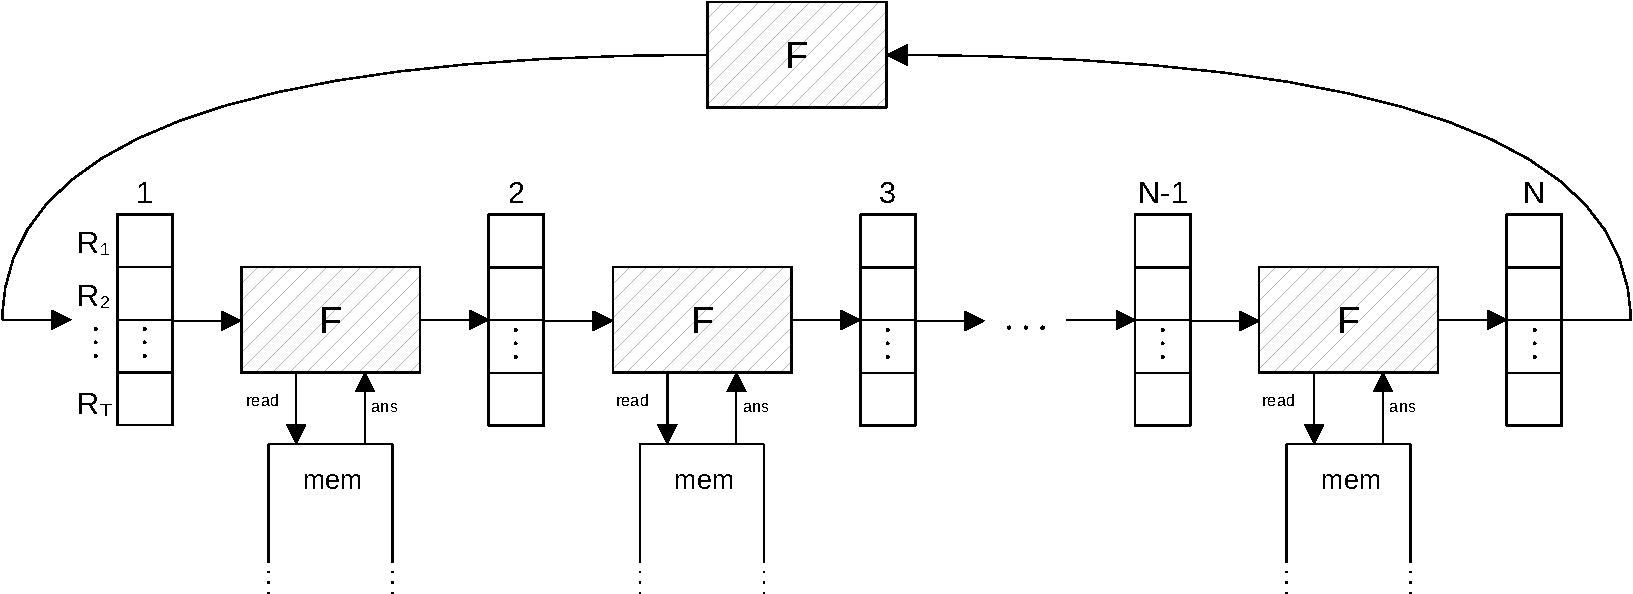
\includegraphics[width=0.8\textwidth]{../figures/computation-memory-diagram}
    \caption{Depiction of our model with $T$ registers and $N$ steps.}
    \label{fig:comp-model}
\end{figure}

Specifically, our model is parameterized by two positive integers $(T, N)$, one representing the number of registers and the other representing the number of steps, and it consists of the following components:
\begin{enumerate}
    \item \textit{Registers}. A constant number $T$ of \textit{registers} $R_1,\dots,R_T$. Registers are a set of accessible cells that are available and can be manipulated by our machine in each state transition. Each of them contains data that, unless stated otherwise, is represented by an element in $\FF$. We use $r_{i,j}$ to denote the field element that, at step $i$, is contained in register $R_j$, with $i\in[N]$ and $j \in [T]$. 
    % \begin{enumerate}[a)]
        % \item \textit{Address}: A unique, distinguishable locator equivalent to a natural number.
        
        % \item \textit{Data}: Piece of information contained within a register. Unless stated otherwise, it will hold an element in $\FF$.
        % \end{enumerate}
    
    \item \textit{Memory}. Memory is the primary location from which the information is retrieved. The main difference between the memory and the registers is that while the memory cells can only store data, the registers can be manipulated by the machine. The memory is represented by an $N \times T$ matrix $\M = \{m_{i,j}\}_{i\in[N],j\in[T]}$ of field elements. At each step, the machine reads the corresponding row of $\M$ (that is, $T$ elements) by ``popping'' it off the memory and using it to compute the next step. 
    \begin{remark}
        Notice that since our machine is read-only, the elements that are read from memory are never ``pushed'' back.
    \end{remark}
    
    % \item \textit{The Program Counter}. Every register machine will contain a special register called the program counter (PC), which tells the machine what is the next instruction to execute.
    
    \item \textit{State Transition Function}. As mentioned before, the \textit{state} of a machine at a given point $i$ consists of the set of $T$ elements from $\FF$ that its registers hold at the $i$-th step of the computation. The machine defines a state transition function $f \colon \FF^{2T} \to \FF^T$ that updates the $i$-th state to the $(i+1)$-th state having as input both the $i$-th state and the data stored in the memory. More concretely, for each step $i \in [N-1]$, the function $f$ satisfies:
    \[
    f(r_{i,1},\dots,r_{i,T},m_{i,1},\dots,m_{i,T}) = (r_{i+1,1},\dots,r_{i+1,T}),
    \]
    and for $i = N$:
    \[
    f(r_{N,1},\dots,r_{N,T},m_{N,1},\dots,m_{N,T}) = (r_{1,1},\dots,r_{1,T}),
    \]
    i.e., $f$ ensures that the state evolves correctly and that it ``cycles back'' from the last state to the first one.
    
    \begin{remark}
        This cyclic relation avoids the need of defining the common notions of inputs and outputs in our model. Moreover, the ordering of our model's states can be shifted in any number of positions and in both directions, so that when we refer to a first or last state we assume that an ordering has been previously fixed.
    \end{remark}
\end{enumerate}

% In the following we refer to the \textit{front-end} of our model as the process of converting a computer program into its equivalent description in terms of our model. More specifically, given a program

\begin{definition}[Arithmetic Circuit]
    An \textit{arithmetic circuit $C$} over a field $\FF$ is a directed acyclic graph in which input and output nodes are connected with intermediate nodes through wires. The nodes are typically called \textit{gates} and are labeled by either $+$ (a \textit{sum} gate) or $\times$ (a \textit{product} gate), with two exceptions. First, every node in it with in-degree zero is called an \textit{input gate} and is labeled by either a variable $x_i$ or an element from $\FF$. Second, every node in it with outdegree zero is called an \textit{output gate} and is labeled by a polynomial with coefficients from $\FF$.
    
    The AC processes its input, hence obtaining a polynomial, in the following way. Starting from the input gates, their path is followed and in the process, some gates compute the sum of the polynomials computed by their children, while product gates compute the product of the polynomials computed by their children. A simple example of this process is illustrated in Fig. \ref{fig:arithmeticCircuit}.
\end{definition}

\begin{figure}[H]
    \centering
    \begin{tikzpicture}
        % vertices
        \node[vertex] (1) at  (0,0) {$+$};
        \node[below left=0.5cm of 1, vertex, fill=cyan!20!white] (A) {$x_1$};
        \node[below right=0.5cm of 1, vertex, fill=cyan!20!white] (B) {$x_2$};
        \node[vertex] (2) at  (2,0) {$\times$};
        \node[right=1.4cm of 2,,yshift=15pt] (F) {Intermediate Gates};
        \node[below right=0.5cm of 2, vertex, fill=cyan!20!white] (C) {$11$};
        \node[right=0.5cm of C] (E) {Input Gates};
        \node[vertex] (3) at  (1,1) {$+$};
        \node[above=0.5cm of 3, rectangle, draw] (D) {$(x_1 + x_2) + 11 \cdot x_2$};
        \node[right=1cm of D] (G) {Output Gates};
        %edges
        \draw[edge] (A) to node[left,xshift=2pt,yshift=4pt]{} (1);
        \draw[edge] (B) to node[right,xshift=0pt,yshift=4pt]{} (1);
        \draw[edge] (B) to node[left,xshift=0pt,yshift=4pt]{} (2);
        \draw[edge] (C) to node[right,xshift=0pt,yshift=4pt]{} (2);
        \draw[edge] (1) to node[right,xshift=0pt,yshift=4pt]{} (3);
        \draw[edge] (2) to node[right,xshift=0pt,yshift=4pt]{} (3);
        \draw[edge] (3) to node[left,xshift=0pt,yshift=4pt]{} (D);
    \end{tikzpicture}
    \caption{Arithmetic circuit that performs two additions and one multiplication.}
    \label{fig:arithmeticCircuit}
\end{figure}


%%%%%%%%%%%%%%%%%%%%%%%%%%%%%%%%%%%%%%%%%%%%%%%%%%%%%%%%%%%%%%%%%%%%%%%%%%%%%%%%
\subsection{Arithmetization: The Bridge Between PIL and our Model}

\begin{table}[H]
    \centering
    \begin{tabular}{|c|l|}
        \hline
        \textbf{PIL Keyword} & \textbf{Register Machine Equivalent} \\\hline
        \tt{namespace} & Defines a new machine. \\\hline
        \tt{pol commit} & Creates a new register. \\\hline
        \tt{pol const} &  \\\hline
        \tt{=} & Defines (a part of) the state transition function. \\\hline
        \tt{pol} &  \\\hline
        \tt{public} &  \\\hline
    \end{tabular}
    \caption{TBD}
    \label{fig:TBD}
\end{table}

In this section, we introduce the basic keywords used in PIL and how they relate to our model. The starting point is the process of \textit{arithmetization} of our model. This means that to arithmetize our model, we must specify the transition function $f$ as a set of polynomial constraints over variables representing the \enquote{current} and the \enquote{next} step of the state.

\begin{definition}[Arithmetization]
    Let $\bar{X}$ be a shorthand for the sequence of formal variables $X_1,\dots, X_T$, $\bar{M}$ a shorthand for the sequence of formal variables $M_1,\dots, M_T$ and $\bar{Y}$ a shorthand for the sequence of formal variables $Y_1\dots, Y_T$. Given a state transition function $f \colon \FF^{2T} \to \FF^T$, the \textit{arithmetization of $f$} consists on computing polynomials $p_1,\dots,p_T \in \FF[\bar{X},\bar{M},\bar{Y}]$ such that for each input state $x \in \FF^{T}$, memory row $m \in \FF^T$ and next state $y \in \FF^T$, we have that:
    \[
    f(x,m) = y \quad \text{ if and only if } \quad p_i(x,m,y) = 0 \text{ for all } i \in [T].	
    \]
    % The aritmetization will be considered to be correct if, given a pair of input $x\in \FF^{2T}$ and output $y \in \FF^T$, we have that $f(x)=y$ if and only if the polynomial constraints get satisfied on this pair.
\end{definition}


% \begin{definition}[execution trace]
    %     The \textit{execution trace} of our model is the matrix of $N \times T$ field elements where:
    %     \begin{enumerate}
        %     \item Each row $i \in [N]$ corresponds with the state of the machine at the $i$-th step.
        
        %     \item Each column $j \in [T]$ corresponds with the content of the $j$-th register over every step.
        %     \end{enumerate}
    % \end{definition}




%%%%%%%%%%%%%%%%%%%%%%%%%%%%%%%%%%%%%%%%%%%%%%%%%%%%%%%%%%%%%%%%%%%%%%%%%%%%%%%%
\subsection{Register Machine Relation}



%%%%%%%%%%%%%%%%%%%%%%%%%%%%%%%%%%%%%%%%%%%%%%%%%%%%%%%%%%%%%%%
\subsection{Related Work}

The main objective of STARK-based languages is translating a computation described as a computer program to a computation described as an AIR. The distinct ways this process can be achieved can be divided into two:
\begin{enumerate}
    \item \textbf{ASIC-like}: This approach is based on writing a computer program in some domain-specific language (DSL) that compiles to an equivalent AIR representing the satisfiability of the computer program. Examples of such are PIL itself and AirScript \cite{AirScript}.
    \item \textbf{CPU-like}: This approach attempts to design an AIR that behaves like a CPU that can handle any computation passed to it. This means that a program is no longer directly compiled into AIR. Instead, the program is compiled to a reduced set of assembly instructions that are understood by the CPU and then the assembly program is transformed to the single AIR representing the correct execution of the CPU. Examples of such are Zilch \cite{EPRINT:MouTso20} and Cairo \cite{EPRINT:GolPapRia21}.
\end{enumerate}

None of the previous variants is the best for every computer program we can think of, as they present several advantages and disadvantages depending on the particular program they are dealing with. Even if more involved, we preferred the ASIC-like approach for PIL for the following reasons:
\begin{enumerate}[a)]
    \item Efficiency: Since the AIR is dependent on the specific computer program, one can design an AIR tailored to that program. In particular, one can decide whether his design is based on a ``wider'' and ``shorter'' or on a ``thinner'' and ``higher'' execution trace.
    \item Modularity: One can divide a program into multiple small pieces (relating these pieces appropriately) and produce an AIR for each piece separately that will ultimately produce an AIR for the entire program. This allows the user to build a vast program through handle (small) logic. 
\end{enumerate}

Similar to PIL, AirScript is a DSL to produce AIR constraints in an ASIC-like fashion. The main problem of AirScript is that it has very little abstraction for describing non-identity constraints. While PIL has built-in keywords for such constraints (that could be augmented in the future), an AirScript user needs to deal with them explicitly: for any argument that is based on random field elements supplied by the verifier during the protocol, a user must define identity constraints attesting the argument's validity by accessing the verifier's randomness. For example, if one wants to produce a program checking that a column is a value in the range $[0,2^4-1]$ by using the Plookup \cite{EPRINT:GabWil20} inclusion argument (in the style described in \cite{EPRINT:PFMBM22}):
\begin{pil}
    namespace Example();
    pol commit a;
    pol constant BITS4;
    
    a in BITS4;
\end{pil}
\begin{pil}
    def Example
    trace_columns:
    main: [a,BITS4,h1,h2]
    aux: [Z]
    
    boundary_constraints:
    enf Z.first = 1
    
    integrity_constraints:
    enf Z'*($rand[0]*(1+$rand[1])+h1+$rand[1]*h2)*($rand[0]*(1+$rand[1])+h2+$rand[1]*h1') = Z*(1+$rand[0])*($rand[1]+a)*($rand[0]*(1+$rand[1])+BITS4+$rand[1]*BITS4')
\end{pil}
Even tho more generic, an AirScript user must choose and understand the argument he wants to deal with, making it less attractive than PIL to the public. 

Regarding CPU-like approaches like Zilch and Cairo, they are both based on a similar workflow: (1) write a program for the computation (either using an assembly-like language directly or using any other language that can be compiled to the CPU bytecode); (2) compile the program to the CPU bytecode; and (3) use a STARK prover for the single AIR to generate a proof. This two-step paradigm suffers from efficiency, as the set of assembly instructions is unlikely to be optimal for every single program. Therefore, while step (3) is independent of the specific program that the user deals with (something that appears to be very handy in proof systems), this does not justify the overhead generated in step (2) as vast programs might have an untractable bytecode whose proof might take too long to compute for practical deployment.
